\documentclass{article}
\usepackage[utf8]{inputenc}
\setcounter{secnumdepth}{0}
\usepackage{graphicx}

\title{Proyecto de Simulación: Simulación de Eventos Discretos}


\begin{document}
\begin{titlepage}
    \centering
{\bfseries\Huge Proyecto de Simulación: Simulación de Eventos Discretos \par}
\vspace{2cm}
\begin{itemize}
    \item {\large Carlos Arturo Pérez Cabrera C-412}
    \item {\large Diana Laura Pérez Trujillo C-412}
\end{itemize}

\end{titlepage}

\section{Introducción}

El objetivo de este proyecto es modelar y analizar el comportamiento de una compañía de seguros, simulando eventos como la llegada de reclamaciones por parte de los clientes asegurados, pérdida de clientes en la empresa o la llegada de nuevos. De forma puntual, se quiere determinar si bajo ciertas condiciones de los parámetros anteriormente mencionados, la compañía cae o no en bancarrota. Se comenzará con un número inicial de clientes n0 y un capital inicial a0 (mayor o igual a 0). A través de simulaciones, se estimará el tiempo en el cual la compañía llega a un estado de bancarrota, es decir, cuando el capital disponible es insuficiente para cubrir las reclamaciones y gastos operativos.

\subsection{Variables que describen el problema}
\begin{itemize}
    \item $n_0$: Número inicial de asegurados en la compañía de seguros.
    \item $a_0$: Capital inicial de la compañía de seguros.
    \item $n$: Número de clientes de la compañía de seguros en un tiempo dado.
    \item $a$: Capital de la compañía de seguros en un tiempo dado.
    \item $v$: Tasa de llegada de nuevos clientes a la empresa de seguros.
    \item $M$: Distribución común que modela la generación de reclamaciones por parte de los asegurados.
    \item $F$: Distribución que modela los montos de reclamación.
    \item $\mu$: Distribución que modela el tiempo que cada asegurado existente permanece con la compañía.
    \item $c$: Tasa fija que los asegurados pagan a la compañía de seguros por unidad de tiempo.
    \item $T$: Duración de la Simulación.
    \item $\lambda$: Tasa de llegada de reclamaciones.
\end{itemize}

\section{Detalles de la Implementación}

\subsection{Distribuciones escogidas}
Luego de un análisis de como debiera ser el comportamiento de cada uno de los eventos (llegada de clientes, llegada de reclamaciones, etc.) se escogieron las siguientes Distribuciones para realizar la simulación:
\begin{itemize}
    \item Llegada de nuevos clientes: Se eligió la distribución de Poisson debido a que la tasa de llegada de nuevos clientes se considera constante o varía poco a lo largo del tiempo, donde el parámetro $v$ representa la tasa de llegada de los clientes por unidad de tiempo.
    \item Cantidad de reclamaciones: Igualmente se escogió la Distribución de Poisson por el motivo anterior.
    \item Costo de las Reclamaciones: Se ha utilizado la distribución de Weibull pues esta permite modelar costos que pueden ser asimétricos y con colas pesadas.
    \item Tasa de retención de los clientes: Se ha escogido la Distribución Exponencial debido a su simplicidad y a que se ajusta bien a la aleatoriedad del tiempo que los clientes permanecen con la empresa.
    El parámetro $m$ de la distribución exponencial representa la tasa promedio de abandono de clientes.

\end{itemize}
 \subsection{Pasos seguidos para realizar la Implementación}
 \begin{itemize}
    \item \underline{Definir las variables y parámetros:} Es necesario identificar y definir las variables y parámetros relevantes del problema, como el número inicial de asegurados, el capital inicial, las distribuciones de reclamaciones y tiempos, la tasa de llegada de nuevos clientes y la tasa fija de pago, entre otros.
    \item \underline{Generar las distribuciones:} Utilizando las distribuciones definidas, se deben generar las reclamaciones y los tiempos de permanencia de los asegurados existentes. Esto se puede hacer utilizando funciones o métodos adecuados según la distribución elegida.
    \item \underline{Simulación del tiempo de bancarrota:} Mediante un bucle o ciclo, se realizarán iteraciones para simular el paso del tiempo y evaluar el estado financiero de la compañía en cada período. Se calculará el capital disponible en cada paso, teniendo en cuenta los ingresos generados por los asegurados existentes y los gastos en reclamaciones.
    \item \underline{Estimación del tiempo de bancarrota:} Durante la simulación, se deben monitorear los cambios en el capital disponible y determinar cuándo la compañía alcanza un estado de bancarrota. Esto puede basarse en una condición específica, como cuando el capital disponible cae por debajo de un umbral predefinido.
    \item \underline{Recopilación de resultados:} Durante la simulación, se deben recopilar los resultados relevantes, como el tiempo en el que se alcanza la bancarrota en cada iteración, el tiempo promedio de bancarrota y la desviación estándar de los tiempos de bancarrota.
    \item \underline{Análisis de resultados:} Una vez finalizada la simulación, se deben analizar los resultados obtenidos. Esto puede implicar calcular la media y la desviación estándar de los tiempos de bancarrota, realizar gráficos para visualizar la distribución de los resultados y realizar comparaciones entre diferentes escenarios o configuraciones de variables.
 \end{itemize}

 \subsection{Descripción de archivos y métodos implementados}
 Para la realización de la simulación se implementaron diferentes métodos para mayor organización de cada etapa de la simulación. 

 \begin{itemize}
    \item \texttt{simulate\_insurance\_company}: \\
        Parámetros de entrada:
        \begin{itemize}
            \item $n_0$: Número inicial de asegurados en la compañía de seguros.
            \item $a_0$: Capital inicial de la compañía de seguros.
            \item $lamb$: Tasa de llegada de reclamaciones de clientes existentes (distribución de Poisson).
            \item $c$: Tarifa fija por cliente. 
            \item $v$: Tasa de llegada de nuevos clientes (distribución de Poisson).
            \item $m$: Parámetro de escala para la tasa de retención de clientes existentes (distribución exponencial).
            \item $weib\_a$: Parámetro de forma para la distribución de costes de reclamación (distribución de Weibull).
            \item $T$: Tiempo máximo de simulación.
        \end{itemize}
        Esta función simula las operaciones de una compañía de seguros durante un tiempo específico. La función devuelve el tiempo en el que la empresa quiebra (si ocurre antes de T) y la matriz que contiene el capital de la empresa en cada paso de tiempo.
        En cada iteración (paso de una unidad de tiempo) la función realiza las siguientes acciones:
        \begin{itemize}
            \item Genera el número de reclamaciones de clientes existentes utilizando la distribución de Poisson con parámetro $lamb$.
            \item Genera el coste de cada reclamación utilizando la distribución de Weibull con parámetro $weib\_a$.
            \item Calcula el ingreso total de las cuotas de los clientes $(n * c)$.
            \item Calcula el gasto total de las reclamaciones.
            \item Genera el número de nuevos clientes utilizando la distribución de Poisson con parámetro $v$.
            \item Simula la retención de clientes existentes utilizando la distribución exponencial con parámetro $m$.
            \item Actualiza el número de clientes ($n$) y el capital de la compañía ($a$) en función de los ingresos, los gastos, los nuevos clientes y los clientes retenidos.
            \item Añade el capital actual a una matriz $a\_array$ para su seguimiento.
        \end{itemize}
    \item \texttt{estimate\_bankruptcy\_time}: \\
    Parámetros de entrada:
    \begin{itemize}
        \item $n_0$: Número inicial de asegurados en la compañía de seguros.
            \item $a_0$: Capital inicial de la compañía de seguros.
            \item $lamb$: Tasa de llegada de reclamaciones de clientes existentes (distribución de Poisson).
            \item $c$: Tarifa fija por cliente. 
            \item $v$: Tasa de llegada de nuevos clientes (distribución de Poisson).
            \item $m$: Parámetro de escala para la tasa de retención de clientes existentes (distribución exponencial).
            \item $weib\_a$: Parámetro de forma para la distribución de costes de reclamación (distribución de Weibull).
            \item $T$: Tiempo máximo de simulación.
            \item $std\_threshold$: Umbral de desviación estándar para los tiempos de quiebra.
    \end{itemize}
    Ejecuta repetidamente la función \texttt{simulate\_insurance\_company} hasta que se cumple un determinado criterio:\\

    1-Se ha ejecutado un número mínimo de simulaciones (al menos 30 en este caso).\\
    2-La desviación estándar de los tiempos de quiebra en todas las simulaciones está por debajo del $std\_threshold$. Esto asegura un cierto nivel de variabilidad en los resultados.

    La función entonces calcula y devuelve el tiempo medio de quiebra, la desviación estándar de los tiempos de quiebra, el número total de iteraciones necesarias y una matriz que contiene las matrices de capital para todas las simulaciones.

    \item \texttt{plot\_ex}: \\ 
         Parámetros de entrada:
         \begin{itemize}
            \item $variable$: Nombre de la variable que se está graficando (utilizado para el título).
            \item $value$: Valor de la variable para esta simulación específica.
            \item $amounts$: Una matriz que contiene el capital de la empresa en cada paso de tiempo para múltiples simulaciones.
         \end{itemize}
         La función itera a través de cada simulación en la matriz $amounts$ y grafica los valores de capital a lo largo del tiempo. A continuación, muestra la gráfica con etiquetas y un título que indica la variable y su valor.

    \item \texttt{execute}: \\
           Función central que actúa como contenedor de las demás funciones y realiza las siguientes funcionalidades: 
           \begin{itemize}
            \item Llama a \texttt{estimate\_bankruptcy\_time} para realizar simulaciones y obtener estadísticas.
            \item Llama a \texttt{plot\_ex} para visualizar el capital de la empresa a lo largo del tiempo para este conjunto específico de parámetros.
            \item Calcula el capital medio en todas las simulaciones en cada paso de tiempo.
            \item Almacena la serie de capital medio en una lista $comparative$.
            \item Muestra en consola la media, la desviación estándar y el número de iteraciones de la función \texttt{estimate\_bankruptcy\_time}.
           \end{itemize}
    \item \texttt{compare}: \\
    Esta función toma una lista de etiquetas como entrada. Asume que la lista $comparative$ contiene múltiples series de capital medio de diferentes simulaciones. es utilizada para hacer una comparación final de los resultados. 
 \end{itemize}
 Todas estas funciones se encuentran dentro del archivo \texttt{sim\_functions.py}.\\
 En los archivos \texttt{test\_lambda.py}, \texttt{test\_v.py} y \texttt{test\_weib\_a.py} se encuentran los llamados a los métodos de la simulación, con diferentes casos prueba, variando los respectivos parámetros: $lamb$, $v$ y $weib\_a$.\\
 En el archivo \texttt{extra\_distributions\_functions.py} se encuentran funciones similares a las descritas en \texttt{sim\_functions.py} pero utilizando diferentes distribuciones a las escogidas inicialmente. Esto se realizó con fines experimentales para observar qué tanto cambiaba la simulación. Se realizó variando el parámetro $lamb$ pues es el que su variación más cambios aporta al comportamiento. 

 \section{Resultados y Experimentos}
 Se realizaron varias simulaciones, donde se variaban diferentes parámetros, en este caso: $lamb$, $v$ y $weib\_a$. La variable de interés que se desea observar es $a$, representando el capital de la compañía de seguros. Específicamente se quiere observar si la compañía de seguros cae o no en bancarrota, bajo ciertas condiciones y diferentes valores de los parámetros. \\
 Las Simulaciones se realizarán hasta que el valor $a$ llegue debajo de cero, o que se alcance un tiempo máximo sin que esto suceda. 

 \subsection{Análisis de comportamiento variando el parámetro lamb}
 El parámetro $lamb$ representa la tasa de llegada de las reclamaciones de los clientes a la empresa de seguros. Se realizaron 4 ejemplos diferentes, donde una ligera variación del parámetro $lamb$ ocasiona una diferencia significativa del comportamiento de la compañía. 
 Para visualizar mejor, se adjuntan los gráficos correspondientes a cada uno de los casos.

 \subsubsection{Ejemplo 1}
 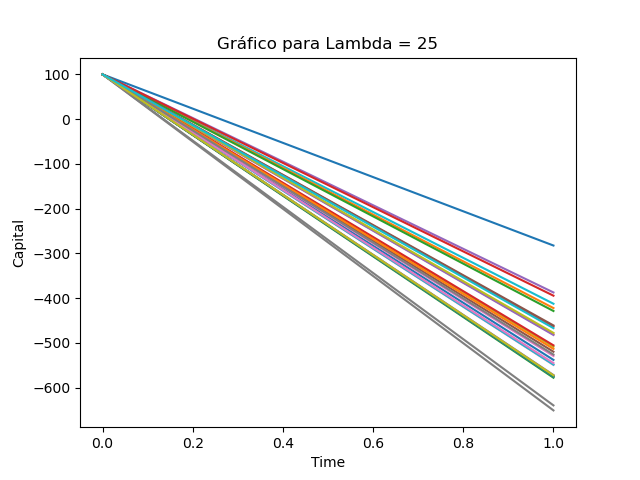
\includegraphics[scale = 0.8]{lamb1.png}
 En este caso, se observa una tendencia a la disminución del capital de la empresa de seguros, hasta caer en la bancarrota.\\

 \subsubsection{Ejemplo 2}
 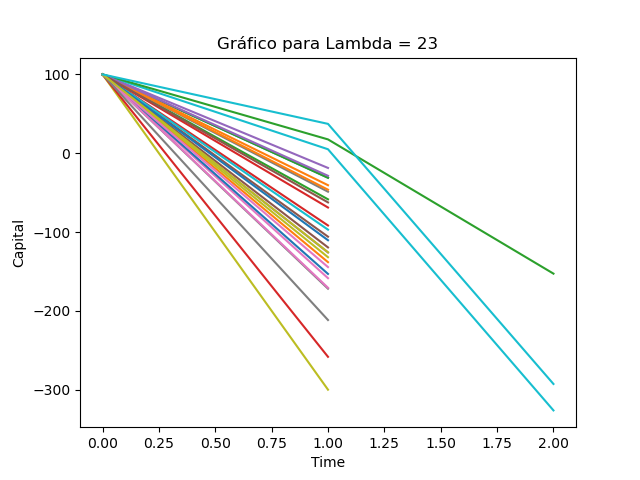
\includegraphics[scale = 0.8]{lamb2.png}
 Este gráfico indica que la compañía de seguros tiene un alto riesgo de caer en bancarrota. La tendencia general del capital es descendente. Las fluctuaciones en el capital podrían ser causadas por eventos aleatorios, como la llegada de grandes reclamaciones o la pérdida de clientes.\\

 \subsubsection{Ejemplo 3}
 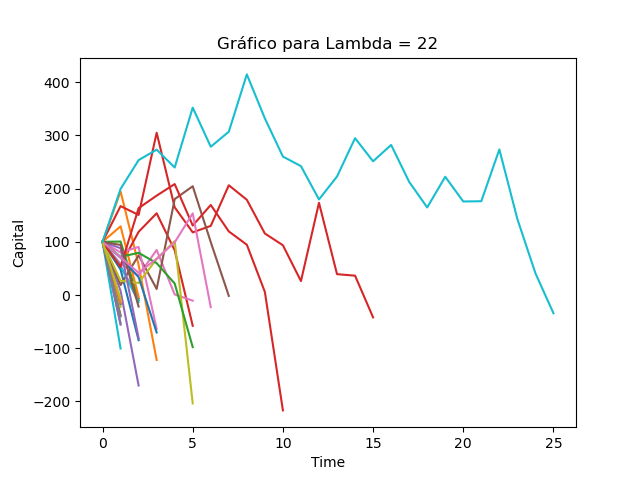
\includegraphics[scale = 0.8]{lamb3.png}
 El capital de la compañía de seguros disminuye a lo largo del tiempo, sin embargo se observan más fluctuaciones y picos que en los ejemplos anteriores, en algunos casos el capital tiene una fuerte tendencia a la disminución, y en otros primero se incrementa, con algunas fluctuaciones hasta finalmente decaer completamente. \\

 \subsubsection{Ejemplo 4}
 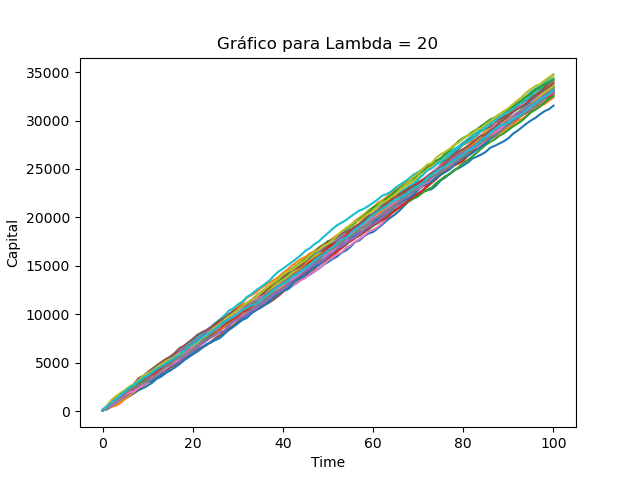
\includegraphics[scale = 0.8]{lamb4.png}
 En este ejemplo, la tendencia del capital de la empresa es creciente, hasta un tiempo máximo definido. 
 Se pudieran usar herramientas estadísticas para predecir si eventualmente la empresa caerá en bancarrota o no, a partir de los datos que ya se han recopilado. La idea que se tuvo inicialmente fue realizar Regresión Logística para ello. 

 \subsubsection{Gráfico Comparativo de los Diferentes Casos}
 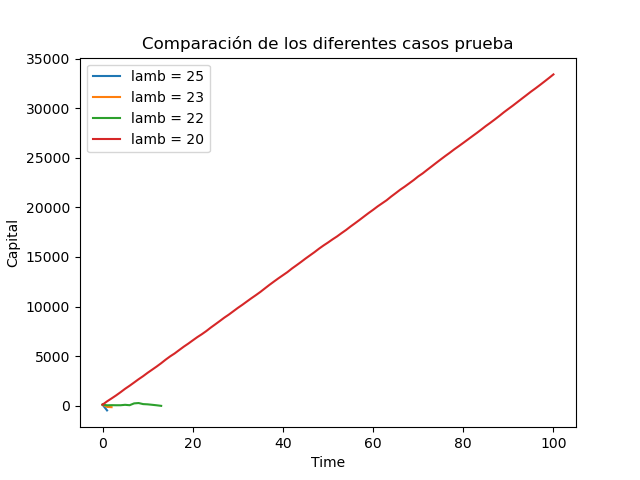
\includegraphics[scale = 0.8]{lambcompare.png}


 \subsection{Análisis de comportamiento variando el parámetro v}

 \subsubsection{Ejemplo 1}
 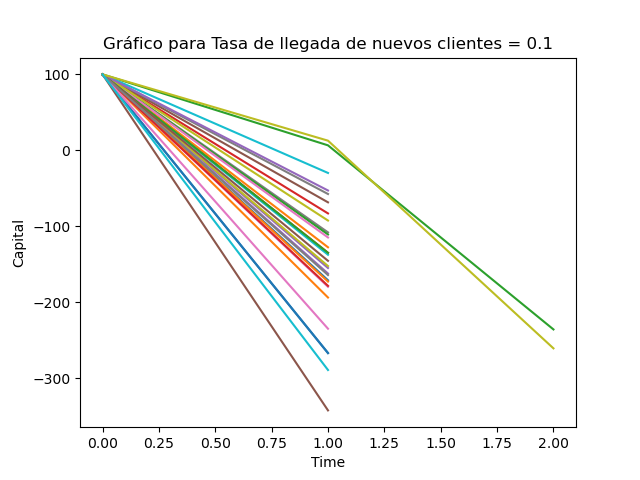
\includegraphics[scale = 0.8]{v1.png}

 \subsubsection{Ejemplo 2}
 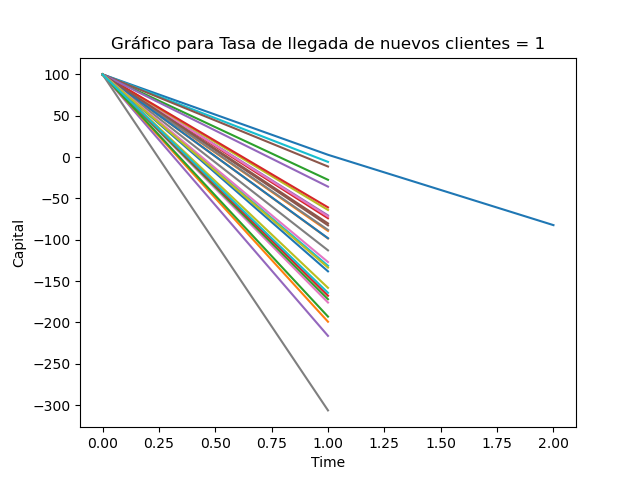
\includegraphics[scale = 0.8]{v2.png}

 \subsubsection{Ejemplo 3}
 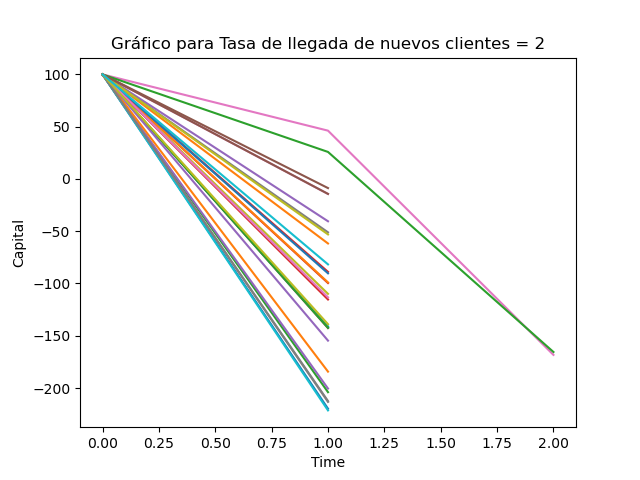
\includegraphics[scale = 0.8]{v3.png}

 \subsubsection{Ejemplo 4}
 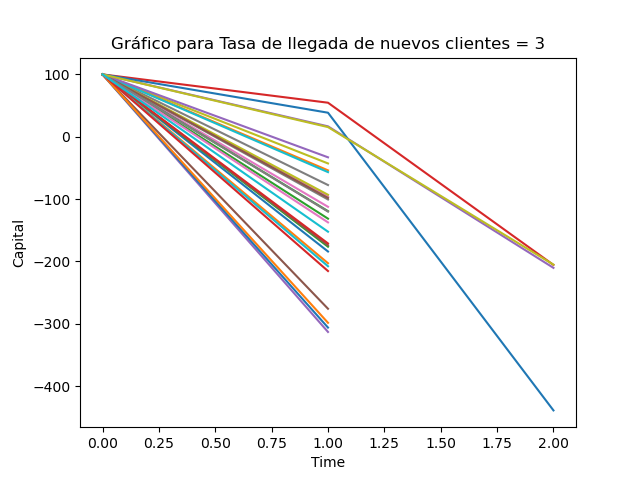
\includegraphics[scale = 0.8]{v4.png}

 \subsubsection{Gráfico Comparativo de los Diferentes Casos}
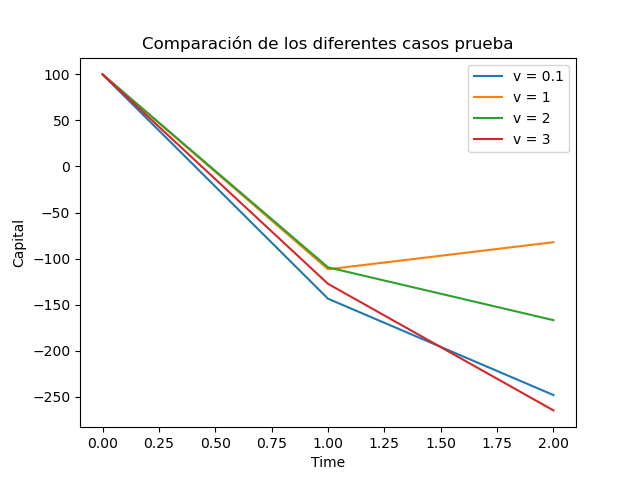
\includegraphics[scale = 0.8]{vcomp.png}

En estos casos, se ha variado la tasa de llegada de nuevos clientes a la compañía de seguros, manteniendo una tasa de llegada de reclamaciones fija ($lamb$=23). Se observa en los cuatro casos, un comportamiento bastante similar en cuanto al decrecimiento del capital. 

\subsection{Análisis de comportamiento variando el parámetro weib\_a}

\subsubsection{Ejemplo 1}
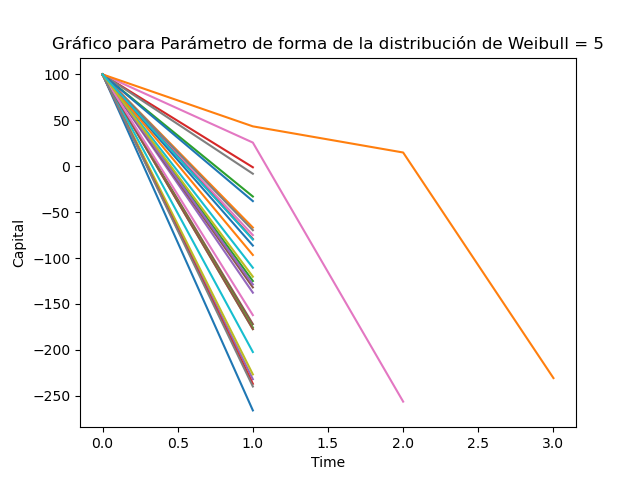
\includegraphics[scale = 0.8]{weib1.png}

\subsubsection{Ejemplo 2}
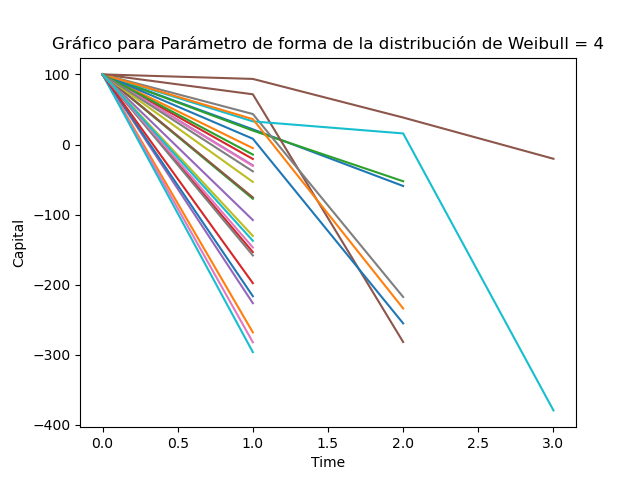
\includegraphics[scale = 0.8]{weib2.png}

\subsubsection{Ejemplo 3}
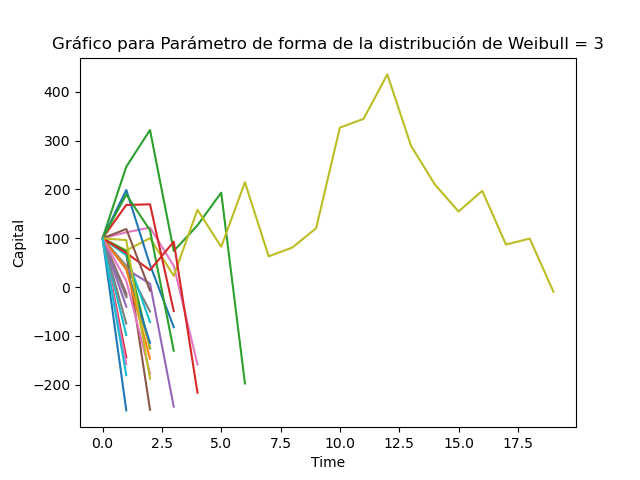
\includegraphics[scale = 0.8]{weib3.png}

\subsubsection{Ejemplo 4}
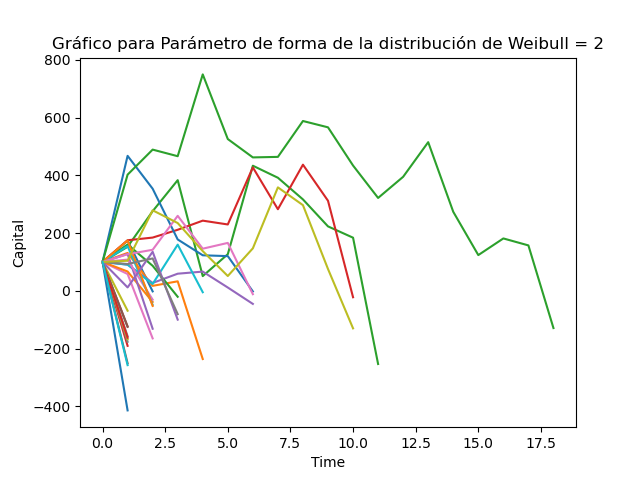
\includegraphics[scale = 0.8]{weib4.png}

\subsubsection{Gráfico Comparativo de los Diferentes Casos}
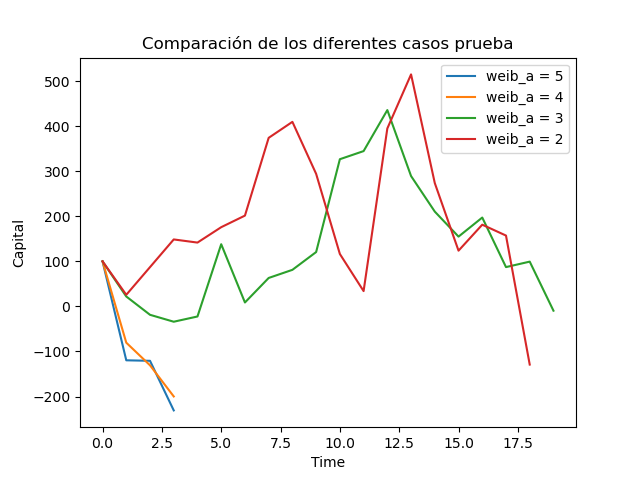
\includegraphics[scale = 0.8]{weibcomp.png}

En estos casos se varía la tasa de costos de las reclamaciones, a mayor valor, más rapido la compañía cae en bancarrota, siendo el caso $weib\_a$ = 2 el que más demora en caer a 0.\\

\subsection{Observaciones}
La variación de la tasa de llegada de las reclamaciones es determinante en el comportamiento del capital de la compañía, cayendo en bancarrota en 3 de los 4 casos probados. En otros casos, no ilustrados, se obtuvo valores grandes en cuanto al crecimiento del capital, utilizando valores muy pequeños del parámetro $lamb$. \\
Por otro lado, se observa que a menor tasa de costo de las reclamaciones, más estable se comporta el capital de la empresa, demorando más la decadencia a 0 del mismo. \\
La variación de la llegada de los nuevos clientes, no aportó cambios significativos al comportamiento del capital. \\

\subsection{Selección de otras Distribuciones}
Se realizó un análisis, variando alguna de las distribuciones definidas inicialmente. 
Para la llegada de las reclamaciones se cambió a una Distribución Normal y para los costos de las mismas se utilizó una Dsitribución Gamma. 
Se analiza el comportamiento del capital de la compañía de seguros, haciendo variar la tasa de llegada de las reclamaciones (parámetro lamb), debido a que anteriormente fue el que más cambios aportó entre los ejemplos. 

\subsubsection{Ejemplo 1}
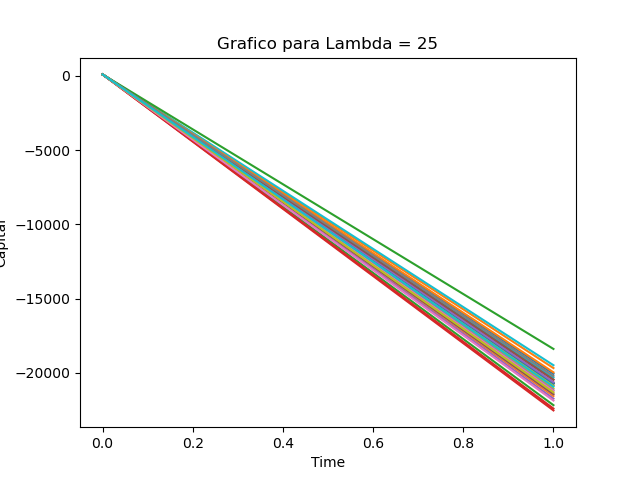
\includegraphics[scale = 0.8]{dis1.png}

\subsubsection{Ejemplo 2}
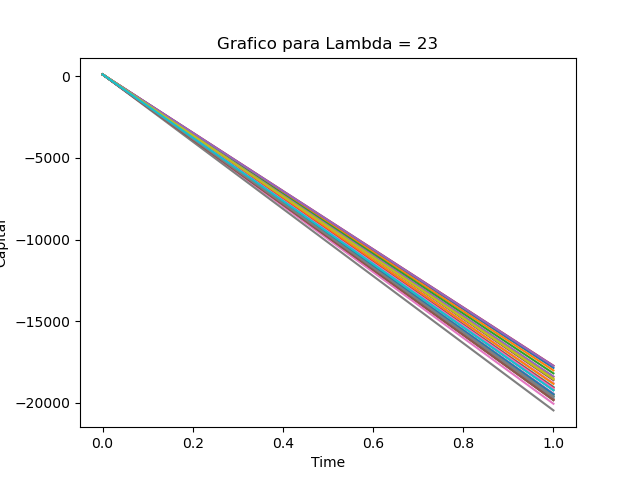
\includegraphics[scale = 0.8]{dis2.png}

\subsubsection{Ejemplo 3}
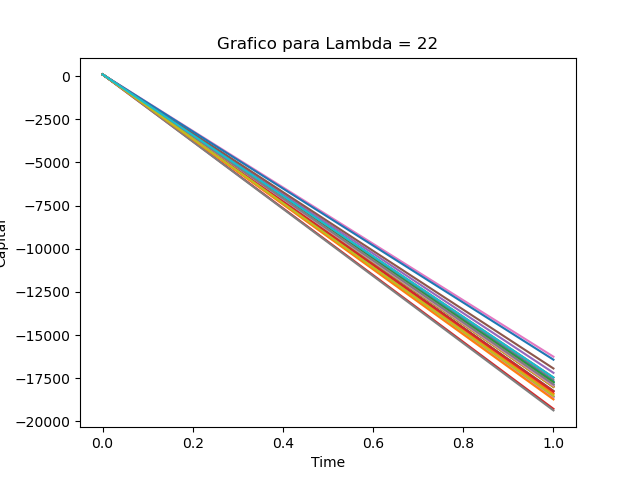
\includegraphics[scale = 0.8]{dis3.png}

\subsubsection{Ejemplo 4}
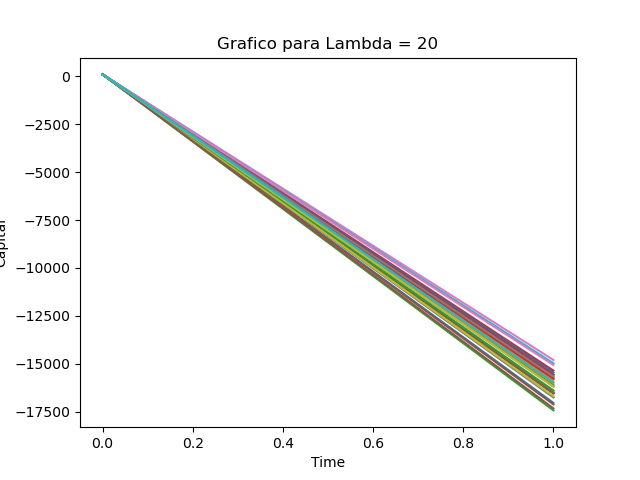
\includegraphics[scale = 0.8]{dis4.png}

\subsubsection{Gráfico Comparativo de los Diferentes Casos}
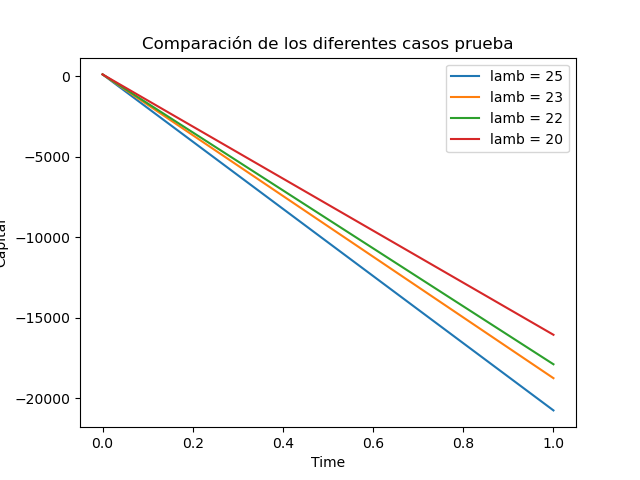
\includegraphics[scale = 0.8]{dicomp.png}

En estos casos, el comportamiento es bastante similar, con una fuerte tendencia decreciente. Se quería observar qué tanto influía la selección de la Distribución adecuada o que mejor describiera el problema en el resultado del comportamiento del capital.
A pesar de que se esocgió variar la tasa de llegada de las reclamaciones, se podría observar también variando los otros parámetros anteriormente analizados. 

\end{document}